% week11_tue_relations.tex -- DSCT Week 11 Tuesday, Oct 27 2026.
% Sources: week-11/instructor/tuesday-run-of-show.md, week-11/README.md,
% week-11/student/tuesday-activity.md, lessons/09-relations.md.
% Every count below was recomputed by brute force in Python (all relations on
% n = 2, 3, 4 elements tested against the property definitions).
\documentclass[aspectratio=169,10pt]{beamer}
\usetheme{Madrid}
\usepackage{tikz}
\usepackage{amssymb}
\title{Does the Relation Earn Its Label?}
\subtitle{Week 11 Tuesday --- Relations, equivalence, and partial orders}
\author{COMSC 2043 \textbullet\ Discrete Structures and Critical Thinking}
\date{October 27, 2026}
\begin{document}

\frame{\titlepage
\note{75 minutes. Spine: Sources, Rules/Assumptions, Work, Check, One-Sentence Summary. Theme for the day: a name is a claim, and a claim needs a witness. Never accept ``it feels symmetric.'' Ask for the pair.}}

\begin{frame}{Today's destination}
\begin{itemize}
\item Say what a relation \emph{is}: a set of ordered pairs.
\item Test four properties one at a time, with a witness or a counterexample.
\item Tell an \textbf{equivalence relation} from a \textbf{partial order}.
\item Catch a confident AI claiming a property it does not have.
\end{itemize}
\note{Run of show: 0:00 AI Fluency (8). 0:08 definitions (14). 0:22 divisibility model (18). 0:40 student activity (14). 0:54 compare criteria, checkpoint (13). 1:07 exit ticket and preview (18, includes slack).}
\end{frame}

\begin{frame}{Warm-up: which of these is ``the same as''?}
\begin{enumerate}
\item ``is friends with''
\item ``has the same birthday as''
\item ``is a sibling of''
\item ``beats'' in rock--paper--scissors
\end{enumerate}
\vspace{4pt}
Gut check, hands up: for each one, is it a fair kind of ``sameness''? Then name \emph{one pair} that breaks it.
\note{Do this before any definitions. Expected: (1) friends: friend of a friend need not be a friend, so transitivity fails. (2) same birthday: works, it sorts people into 366 bins. (3) sibling: you are not your own sibling, so reflexivity fails (and half-siblings depending on definition). (4) beats: rock beats scissors, scissors beats paper, paper beats rock. A cycle. Not transitive, not reflexive, not symmetric. Let students argue; do not resolve it, the next slides give the vocabulary.}
\end{frame}

\begin{frame}{AI Fluency: a confident, untested label}
\begin{block}{An AI says}
``Divisibility is \emph{symmetric}, because $2$ divides $6$.''
\end{block}
\begin{itemize}
\item What would symmetric actually require?
\item Which single pair tests the claim?
\item Write the missing property in one line.
\end{itemize}
\note{Eight minutes total for warm-up plus this. Target: symmetric means for every (a,b) in R, (b,a) is in R. The AI showed one pair going forward and never checked the reverse. Test: does 6 divide 2? No. So (2,6) is in R and (6,2) is not. One counterexample kills the claim. Evidence for ``for all'' needs a proof; evidence against needs one witness.}
\end{frame}

\begin{frame}{What a relation is}
A \textbf{relation} $R$ on a set $S$ is a set of ordered pairs $R \subseteq S\times S$.
\begin{itemize}
\item $a\,R\,b$ means $(a,b)\in R$. Order matters: $(2,6)\neq(6,2)$.
\item Three ways to write the same thing: \emph{list the pairs}, a \emph{matrix}, a \emph{digraph}.
\item Name the domain $S$ first. If the domain drifts, the answer changes.
\end{itemize}
\vspace{4pt}
\textbf{Counting is humbling:} on just 3 elements there are $2^9=512$ different relations.
\note{Why 512: S x S has 9 ordered pairs and each is in or out. On 2 elements: 16. On 4 elements: 65,536. Most of them are junk; the interesting ones have structure, and the four properties are how we describe structure. Quick poll: how many relations on a 4-element set? ($2^{16}$.)}
\end{frame}

\begin{frame}{The four properties, as questions}
\begin{tabular}{@{}ll@{}}
\textbf{Reflexive} & Does every $a$ relate to itself? $(a,a)\in R$ for all $a$ \\[3pt]
\textbf{Symmetric} & Does every forward pair have a reverse? $(a,b)\Rightarrow(b,a)$ \\[3pt]
\textbf{Antisymmetric} & Do two-way pairs only happen for $a=b$? $(a,b)\wedge(b,a)\Rightarrow a=b$ \\[3pt]
\textbf{Transitive} & Do chains shortcut? $(a,b)\wedge(b,c)\Rightarrow(a,c)$ \\
\end{tabular}
\vspace{8pt}
\begin{itemize}
\item To say \textbf{yes}: check \emph{every} pair. To say \textbf{no}: show \emph{one} witness.
\item Symmetric and antisymmetric are not opposites. Both can hold; neither can hold.
\end{itemize}
\note{Both hold: equality, R = {(1,1),(2,2)}. Neither: R = {(1,2),(2,1),(1,3)} on {1,2,3}: not symmetric because (1,3) lacks (3,1); not antisymmetric because of (1,2),(2,1). Ask students to build their own ``both'' and ``neither'' examples if time.}
\end{frame}

\begin{frame}{Model: divisibility on $S=\{1,2,3,6\}$}
\begin{columns}[T]
\begin{column}{0.48\textwidth}
$a\,R\,b$ when $a$ divides $b$.\\[4pt]
Pairs (9 of them):\\
$(1,1),(1,2),(1,3),(1,6),$\\
$(2,2),(2,6),(3,3),(3,6),(6,6)$
\vspace{6pt}

Matrix (row $a$, column $b$):
\[
\begin{array}{c|cccc}
 & 1&2&3&6\\\hline
1&1&1&1&1\\
2&0&1&0&1\\
3&0&0&1&1\\
6&0&0&0&1
\end{array}
\]
\end{column}
\begin{column}{0.48\textwidth}
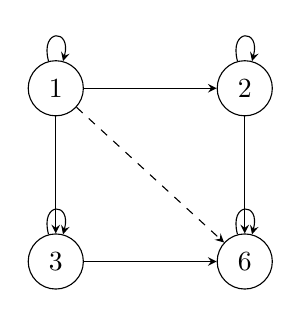
\begin{tikzpicture}[>=stealth,node distance=2cm,every node/.style={circle,draw,minimum size=7mm}]
\node (1) at (0,0) {1}; \node (2) at (2.4,0) {2};
\node (3) at (0,-2.2) {3}; \node (6) at (2.4,-2.2) {6};
\draw[->] (1) -- (2); \draw[->] (1) -- (3); \draw[->] (2) -- (6); \draw[->] (3) -- (6);
\draw[->,dashed] (1) -- (6);
\foreach \n in {1,2,3,6} {\draw[->] (\n) to[loop above,looseness=6] (\n);}
\end{tikzpicture}
\end{column}
\end{columns}
\note{Build the pair list live, row by row from the matrix: ask ``which b does 1 divide?'' etc. Digraph: arrows are the pairs. Dashed arrow 1 to 6 is the transitive shortcut; loops are reflexivity. Trace the checks on the next slide off this same picture so the matrix, digraph, and list visibly agree.}
\end{frame}

\begin{frame}{Test each property separately}
\begin{center}
\begin{tabular}{lcl}
\textbf{Property} & \textbf{Holds?} & \textbf{Witness / reason} \\\hline
Reflexive & yes & diagonal of matrix all 1s; $a\mid a$ \\
Symmetric & \textbf{no} & $(2,6)\in R$ but $(6,2)\notin R$ \\
Antisymmetric & yes & no off-diagonal pair is two-way (matrix has no mirrored 1s) \\
Transitive & yes & $(1,2),(2,6)\Rightarrow(1,6)$; all other chains checked \\
\end{tabular}
\end{center}
\vspace{4pt}
\textbf{Verdict:} reflexive + antisymmetric + transitive = a \textbf{partial order}. Not symmetric, so \emph{not} an equivalence relation.
\note{Say the matrix check out loud: symmetric means the matrix equals its mirror across the diagonal. Here 2,6 is a 1 and 6,2 is a 0. Antisymmetric means no off-diagonal 1 is mirrored by another 1. Do not say ``divisibility is a partial order'' in general without the domain: on all integers including negatives and zero it is trickier; on positive integers it is a partial order. State the domain every time.}
\end{frame}

\begin{frame}{Your turn (14 min): Does the relation earn its label?}
Use \texttt{student/tuesday-activity.md}.
\begin{enumerate}
\item Represent $R$ as pairs \textbf{and} as a matrix or digraph.
\item Classify all four properties. Every ``no'' needs a counterexample pair or chain.
\item Equivalence, partial order, neither, or both? Name the required properties.
\item Check: does your matrix/digraph agree with your symmetry and antisymmetry answers?
\end{enumerate}
\textbf{Watch for:} domain drift (using $\{1,2,3,4,5,6\}$ by accident) and reversed pairs ($b\mid a$ instead of $a\mid b$).
\note{Circulate. Common errors: writing (6,2) because ``2 goes into 6'' backwards; calling it transitive without checking a chain; saying ``both'' because it is reflexive. If a pair finishes early: ask them to change the relation to ``a and b have the same remainder mod 2'' on {1,2,3,6} and re-classify. That one is an equivalence relation.}
\end{frame}

\begin{frame}{Equivalence relation vs.\ partial order}
\begin{center}
\begin{tabular}{lcc}
 & \textbf{Equivalence} & \textbf{Partial order} \\\hline
Reflexive & \checkmark & \checkmark \\
Symmetric & \checkmark & --- \\
Antisymmetric & --- & \checkmark \\
Transitive & \checkmark & \checkmark \\\hline
Feels like & \emph{``is the same as''} & \emph{``comes before / sits under''}
\end{tabular}
\end{center}
\begin{itemize}
\item Equivalence \textbf{sorts into bins} (a partition): ``same remainder mod 3'' makes 3 bins.
\item Partial order \textbf{ranks, but not everything is comparable}: $2$ and $3$ do not divide each other.
\end{itemize}
\note{This is the side-by-side slide the run of show asks for. The ``interesting'' fact: every equivalence relation is exactly a partition of the set into bins and vice versa. Count check, verified by brute force: on a 3-element set, of the 512 relations, exactly 5 are equivalence relations (the 5 ways to partition 3 things) and exactly 19 are partial orders. On 4 elements: 65,536 relations, 15 equivalences, 219 partial orders.}
\end{frame}

\begin{frame}{Where you already meet these}
\begin{columns}[T]
\begin{column}{0.48\textwidth}
\textbf{Equivalence = ``same bin''}
\begin{itemize}
\item Same hash $\Rightarrow$ same file contents
\item Same remainder mod $n$ (clocks, checksums)
\item Duplicate detection, grouping records
\end{itemize}
\end{column}
\begin{column}{0.48\textwidth}
\textbf{Partial order = ``must come before''}
\begin{itemize}
\item Prerequisites: which course before which
\item Build order: \texttt{make}, package dependencies
\item Git history: this commit descends from that one
\end{itemize}
\end{column}
\end{columns}
\vspace{6pt}
\textbf{Question for the room:} a course scheduler treats prerequisites as a relation. Which property must it \emph{never} violate to avoid a deadlock?
\note{Answer: a cycle. If A requires B requires C requires A, no valid order exists, which is the same cycle as rock-paper-scissors. Partial orders forbid cycles through antisymmetry plus transitivity. This is the payoff for the warm-up; tie it back explicitly.}
\end{frame}

\begin{frame}{Challenge: how many bins?}
\begin{block}{Puzzle}
Let $S=\{0,1,\dots,11\}$ and $a\sim b$ when $a$ and $b$ have the same remainder mod $4$.
\end{block}
\begin{enumerate}
\item How many bins? How big is each?
\item Is $\sim$ also a partial order? Give the property that fails.
\item Does $a\sim b$ and $b\sim c$ force $a\sim c$? Say why in one sentence.
\end{enumerate}
\note{Answers: 4 bins of 3 each. Not a partial order: antisymmetry fails, since 0 ~ 4 and 4 ~ 0 with 0 not equal to 4. Transitive because equal remainders are an equality, and equality chains. Use as a floater if the activity goes fast, or as a bridge into the checkpoint.}
\end{frame}

\begin{frame}{Reasoning Odyssey Checkpoint 2 (Weeks 8--11)}
\begin{itemize}
\item It \textbf{replaces} this week's Decision Gate. Submit one, not both.
\item Pull from recursion, logic, probability, and relations: what changed in how you check a claim?
\item Use the spine: \textbf{Sources $\to$ Rules $\to$ Work $\to$ Check $\to$ One-Sentence Summary}.
\end{itemize}
\textbf{Plan it now (2 min):} which one earlier claim of yours would you re-examine with a witness or counterexample?
\note{Details live in student/odyssey-checkpoint-2.md. Have students write a one-line checkpoint plan before they leave: which week, which claim, which test.}
\end{frame}

\begin{frame}{Exit ticket (and Thursday)}
Write one claim, one witness:
\begin{block}{}
``Divisibility on $\{1,2,3,6\}$ is \underline{\hspace{2cm}} but not \underline{\hspace{2cm}}, because the pair \underline{\hspace{2cm}} \underline{\hspace{2cm}}.''
\end{block}
\vspace{4pt}
\textbf{Thursday:} Pair Reasoning. Bring a relation classifier, matrix, or digraph, and be ready to argue about it with a partner. The individual Pair Reasoning report is due after.
\note{Model answer: ``reflexive but not symmetric, because the pair (2,6) has no (6,2).'' Collect traces. Thursday run of show is in week-11/instructor/thursday-run-of-show.md.}
\end{frame}

\end{document}
